\begin{frame}{Appendix}
Given a data set of $N$ points $\left\lbrace x_i \right\rbrace_{i=1}^N \subseteq \mathcal{X}$, 
defining a non-linear feature mapping $\Phi$ from $\mathcal{X}$ to a higher dimensional Hilbert space $\mathcal{H}$,

\begin{align}
\label{eq:svc1}
&\min R^2 + \sum c_i\xi_i\\		
\text{subject to}\quad &  \| \Phi(x_j) - g\|^2 \leq R^2 + \xi_j,\; \forall j \nonumber \\
& \xi_j \geq 0 \nonumber
\end{align} 
Introducing the Lagrangian
\begin{align}
\label{eq:svc2}
L=R^2&-\sum_j\left(R^2+\xi_j-\|\Phi(x_j)-g\|^2\right)\beta_j\nonumber\\
     &-\sum\xi_j\mu_j+\sum c_i\xi_j,
\end{align}
$\beta_j\geq 0$ and $\mu_j\geq 0$ are Lagrange multipliers, $c_i$ is the regularization constant.
\end{frame}
\begin{frame}
Two supervised data sets are indicated by users, 
\begin{align*}
\mathcal{X^+}=&\left\lbrace \left( x_l, y_l) \,|\,  x_l \in \mathcal{X}, y_l=1 \right)\right\rbrace\\
\mathcal{X^-}=&\left\lbrace \left( x_r, y_r) \,|\, x_r \in \mathcal{X}, y_r=-1\right)\right\rbrace\\
&l, r \in \left\lbrace 1,\ldots ,N\right\rbrace
\end{align*}
where $\mathcal{X^+}$ is the outlier set, and $\mathcal{X^-}$ is normal set.
\end{frame}
\begin{frame}
An impact function $f$ is defined in the input space $\mathcal{X}$ given $\mathcal{X^+}$ and $\mathcal{X^-}$.  
\begin{gather}
f\left(x_i\right) = \frac{\sum_{x_l\in \mathcal{X^+}}K\left(x_l, x_i\right)}{\sum_l\mathbf{1^+}\left(x_l,x_i\right)} + 
\frac{\sum_{x_r\in \mathcal{X^-}}K\left(x_r, x_i\right)}{\sum_l\mathbf{1^-}\left(x_r,x_i\right)}
\end{gather}
where the kernel function is taken as a similarity measurement, note that
\[
K(x, x_i) = \exp\left(\frac{\| x - x_i \|^2}{-2h^2}\right)
\]
And $\mathbf{1^+}$ and $\mathbf{1^-}$ are both indicator functions defined as
\begin{align*}
\mathbf{1^+}(x_l, x_i)= &
     \begin{cases}
     	1 & \quad \| x_l - x_i \| \leq 2h\\
     	0 & \quad \text{otherwise}
     \end{cases}\\
\mathbf{1^-}(x_r, x_i)=&
     \begin{cases}
     	-1 & \quad \| x_r - x_i \| \leq 2h\\
     	0 & \quad \text{otherwise}
     \end{cases}     
\end{align*}
\end{frame}
\begin{frame}
The regularization weights $c_j$ can be computed
\begin{align}
c_j = \begin{cases}
c_0 \cdot \frac{1-f\left(x_j\right)}{1-\exp\left(-2\right)} + \frac{1}{N}\cdot \frac{f\left(x_j\right) - \exp\left(-2\right)}{1-\exp\left(-2\right)} & \text{if}\quad f\left(x_j\right) > 0\\
c_0 \cdot \frac{1-\left|f\left(x_j\right)\right|}{1-\exp\left(-2\right)} + \frac{\left|f\left(x_j\right)\right| - \exp\left(-2\right)}{1-\exp\left(-2\right)} & \text{if}\quad f\left(x_j\right) < 0
\end{cases}
\end{align}
where $c_0$ is the initial value of $c_j$ and $N$ is the sample size.
\end{frame}
\begin{frame}
Now setting the derivative of the Lagrange $L$ to zero, we have:
\begin{align}
\sum\beta_j=1\\
g=\sum\beta_j\Phi(x_j)\\
\beta_j=c_j-\mu_j
\end{align}  
The KKT conditions again require that
\begin{gather}
\xi_j\mu_j=0\\
\left(R^2+\xi_j-\|\Phi(x_j)-g\|^2\right)\beta_j=0
\end{gather} 
\end{frame}
\begin{frame}
Eliminating the variables $R$, $g$, and $u_j$, the Wolf dual form is obtained, where $\beta_j$ are the only variables.
\begin{gather}
W=\sum_j\Phi(x_j)^2\beta_j-\sum_{i,j}\beta_i\beta_j\Phi(x_i)\cdot\Phi(x_j)\\
\text{subject to}\quad 0\leq\beta_j\leq c_j, \; j=1,\ldots,N. 
\end{gather}
Solve the dual problem, we have found $\left\lbrace \beta_j \right\rbrace$.
\end{frame}
%\begin{frame}{Statistical Implication}
%\begin{block}{Reichenbach's \textit{Common Cause Principle}}
%If $X$ and $Y$ are correlated, then either $X$ causes $Y$ or $Y$ causes $X$ or they share a latent common cause $Z$.
%\end{block}
%\begin{figure}
%\setcounter{subfigure}{0}
%	\centering
%	\begin{subfigure}[H]{0.3\textwidth}
%		\centering
%		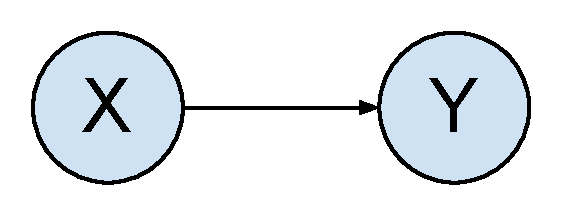
\includegraphics[scale=0.3]{imgs/x2y}
%		\caption{$X$ causes $Y$}
%		%\label{}	
%	\end{subfigure}
%	\begin{subfigure}[H]{0.3\textwidth}
%		\centering
%		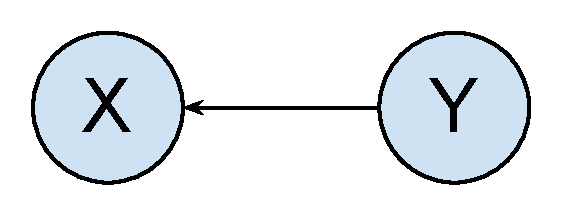
\includegraphics[scale=0.3]{imgs/y2x}
%		\caption{$Y$ causes $X$}
%		%\label{}	
%	\end{subfigure}
%	\begin{subfigure}[H]{0.3\textwidth}
%		\centering
%		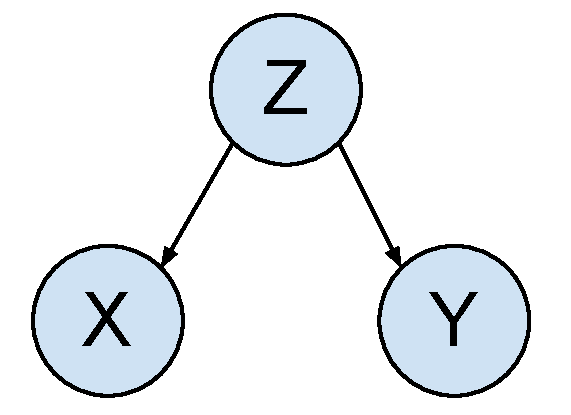
\includegraphics[scale=0.3]{imgs/z2xy}
%		\caption{A common latent cause $Z$}
%		%\label{}	
%	\end{subfigure}
%\end{figure}\pause
%\begin{itemize}
%\item<+-|alert@+> It links causality with probability
%\end{itemize}
%\end{frame}
%\begin{frame}{Functional Causal Model (pearl et al.)} 
%\begin{itemize}[<+->]
%\item A set of variables (factors) $\left\lbrace X_1,\ldots,X_n \right\rbrace$
%\item Directed acyclic graph $\mathcal{G}$ with vertices $\left\lbrace X_1,\ldots,X_n \right\rbrace$
%\item Parents of node $X_i$ in $\mathcal{G}$ are its direct causes
%\item $X_i=f_i(Parents(X_i),\epsilon_i)$, where $\left\lbrace\epsilon_1,\ldots,\epsilon_n\right\rbrace$ are jointly independent noises
%\item The above entails a joint probability distribution $P(X_1,\ldots,X_n)$
%\item Problems are twofold:
%      \begin{enumerate}
%		\item How is the $P$ like?
%		\item Can we recover $\mathcal{G} from P$? 
%	\end{enumerate}
%\item[] \begin{textblock*}{200mm}(0.6\textwidth,-2cm)
%		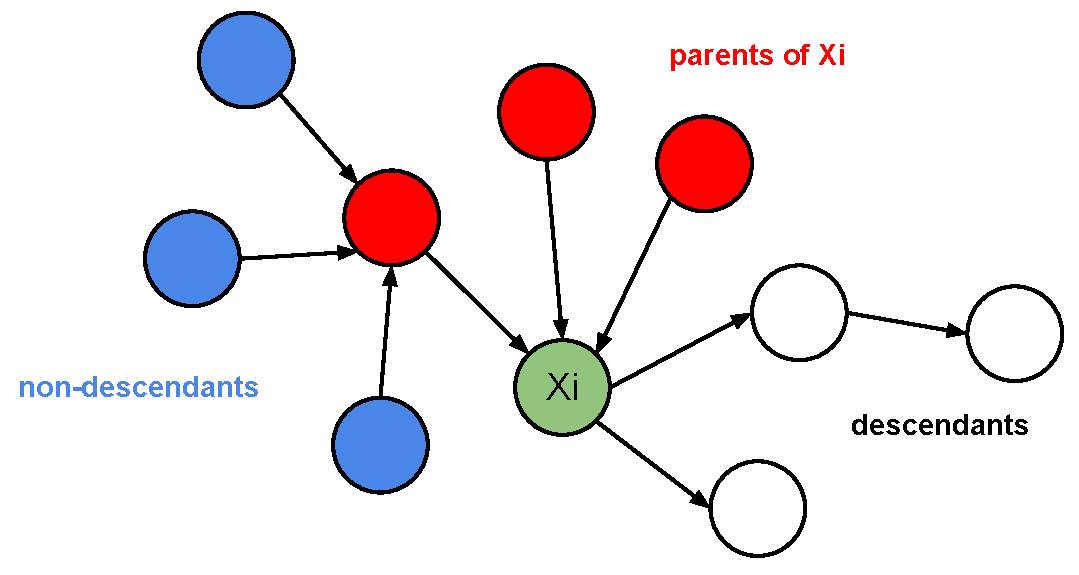
\includegraphics[scale=0.25]{imgs/causalgm}
%	\end{textblock*}
%\end{itemize}
%\end{frame}
%\begin{frame}{Functional Causal Model, ctd.}
%The following are equivalent:
%\begin{itemize}
%\item A functional causal model exists
%\item Local causal Markov condition: $X_i$ is statistically independent of its non-descendants given $X_i$'s parents
%\item Global Causal Markov condition: \textbf{d-separation} characterize the set of independences over all the observables
%\item Factorization: $P(X_1,\ldots,X_n)=\prod_iP(X_i\,|\,Parents(X_i))$
%\end{itemize}
%\end{frame}
%\begin{frame}{Learning causation from Data?}
%\begin{block}{Question}
%Given observational data, can we infer $\mathcal{G}$?
%\end{block}
%\begin{itemize}
%\item \textbf{Simple answer:} impossible without additional information
%\item Possible with interventions (outside force, empirical treatment, etc.)
%\item By conditional independence tests, \textit{Markov equivalence class} containing $\mathcal{G}$ can be learned. \alert{But}, it fails in simplest 2-nodes case.
%\item 2-nodes case can be tackled applying residual dependence test. (see Hoyer et al.)
%\end{itemize}
%\end{frame}
%\begin{frame}{Markov Equivalence Class}
%\textbf{Simplest case with three variables}
%\begin{itemize}
%\item[]<1-> \begin{figure}
%\setcounter{subfigure}{0}
%			\begin{subfigure}[H]{0.4\textwidth}
%			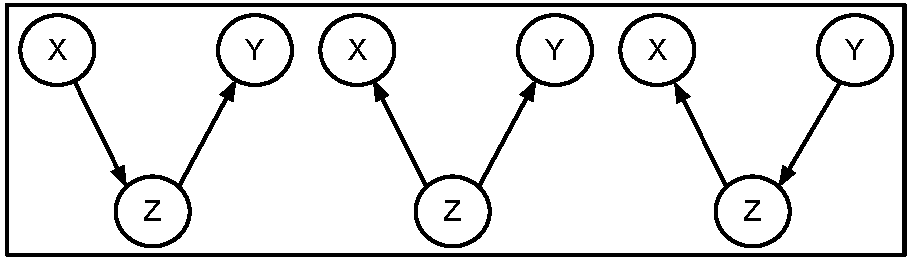
\includegraphics[scale=0.4]{imgs/eqv}
%			\caption{Equivalence}
%			\end{subfigure}\hfill
%			\begin{subfigure}[H]{0.3\textwidth}
%			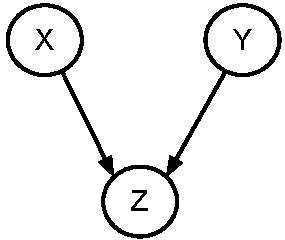
\includegraphics[scale=0.4]{imgs/noneqv}
%			\caption{Non-equivalence}
%			\end{subfigure}
%		\end{figure}
%\item<2-> Samples can be explained by all graphs in equivalence class
%\item<3-> For example:
%\begin{table}
%\centering
%\begin{tabular}{|c|c|}
%\hline
%Equivalence class & Non-equivalence class \\\hline
%$Dep(X,Z\,|\,\emptyset)$ & $Dep(X,Z\,|\,\emptyset)$\\\hline
%$Dep(Y,Z\,|\,\emptyset)$ & $Dep(Y,Z\,|\,\emptyset)$\\\hline
%$Dep(X,Y\,|\,\emptyset)$ & \alert{$Ind(X,Y\,|\,\emptyset)$}\\\hline
%$Ind(X,Y\,|\,Z)$ & \alert{$Dep(X,Y\,|\,Z)$}\\\hline
%\end{tabular}
%\end{table}	
%\end{itemize}
%\end{frame}